\documentclass[12pt,aspectratio=43]{beamer}

% 自訂字體的封包
\usepackage{fontspec}

% 導入圖形與表格的封包
\usepackage{graphicx}
\usepackage{booktabs}

% 排列多個子圖形的封包
\usepackage{subfigure} 

 % 提供進階數學環境與公式排版
\usepackage{mathtools, amsmath, amsfonts, amsthm, latexsym} 

%% 設定中文字體
\usepackage{xeCJK}
\setCJKmainfont[AutoFakeBold=3.5 , AutoFakeSlant=0.2]{標楷體}
\setmainfont{Times New Roman}
\XeTeXlinebreaklocale "zh"
\XeTeXlinebreakskip = 0pt plus 1pt

% 自訂字體顏色的封包
\usepackage{color} 

% 圖表自動編號的封包
\usepackage{caption} 

% 允許表格的一格能多列呈現的封包
\usepackage{multirow} 

% 可指定表格排版的封包
\usepackage{array}

% 翻轉表格的封包
\usepackage{lscape} 

% 序列標號
\usepackage{enumerate} 

%% 設定自動編號
\setbeamertemplate{caption}[numbered]

%% 自訂顏色
\definecolor{Myblue}{RGB}{57,108,144}
\definecolor{Default_Blue}{RGB}{52,51,171}

% (動畫)字會若隱若現的顯示
\beamersetuncovermixins{\opaqueness<1->{45}}{\opaqueness<1->{95}} 

% 設定中文的標籤
\renewcommand{\figurename}{圖}
\renewcommand{\tablename}{表}

% 排版形式 
\mode<presentation>{
\usetheme{CambridgeUS}
% 外框形式
\useoutertheme{shadow}
% enumerate 及 item 的形狀
\setbeamertemplate{itemize items}[triangle]
% 調整外框形式的字體大小
\setbeamerfont{headline}{size=\scriptsize}
\setbeamerfont{footline}{size=\scriptsize}
% 取消右下方的跳轉工具列
\setbeamertemplate{navigation symbols}{} 
% 自定義2：清除外框下緣但僅出頁碼
\setbeamertemplate{footline}[page number] 
% 顏色主題
\usecolortheme{dove}
% 設定頁面邊界
\setbeamersize{text margin left=0.2cm, text margin right=0.2cm}
\special{papersize=\the\paperwidth,\the\paperheight}
\providecommand{\tabularnewline}{\\}
}

\title{\fontsize{24pt}{20pt}統計諮詢與專業實務}
\author{\fontsize{12pt}{0pt}黃丞暘}
\institute{\fontsize{12pt}{0pt}國立東華大學應用數學統計所}
\date{November 20, 2025}

\begin{document}

% 封面
\begin{frame}
  \titlepage
\end{frame}

% PART A.1 問題與目的
\begin{frame}[t]{\textbf{PART A.1}}
\vspace*{10pt}

{
\setlength{\baselineskip}{1.5\baselineskip}
% 問題
{
\Large
\parbox{\linewidth}{\raggedright \textbf{問題}\\
評估三種身體測量對體脂肪的邊際效應與貢獻}
}

\vspace*{2cm}

% 目的
{
\Large \parbox{\linewidth}{\raggedright \textbf{目的}\\
找出哪個測量對體脂肪的影響最大且顯著}
}
}
\end{frame}

% PART A.1 資料
\begin{frame}[t]{\textbf{PART A.1}} 
\vspace*{10pt}
{
\setlength{\baselineskip}{1.3\baselineskip}   % 行距放大 1.3 倍
{
\Large
\parbox{\linewidth}{\raggedright \textbf{資料來源}}
}
}

\begin{itemize}
    \item CH07TA01.txt
  \begin{enumerate}[]
    \setlength{\itemsep}{6pt}
    \item 樣本數：20（25-34歲的健康女性）
    \item 研究變數：$X_1$：Triceps(mm)，$X_2$：Thigh(cm)，$X_3$：Midarm(cm)
    \item 目標變數：$Y$：bodyfat(\%)
  \end{enumerate}
\end{itemize}

    \begin{figure}
      \hspace{0cm}
      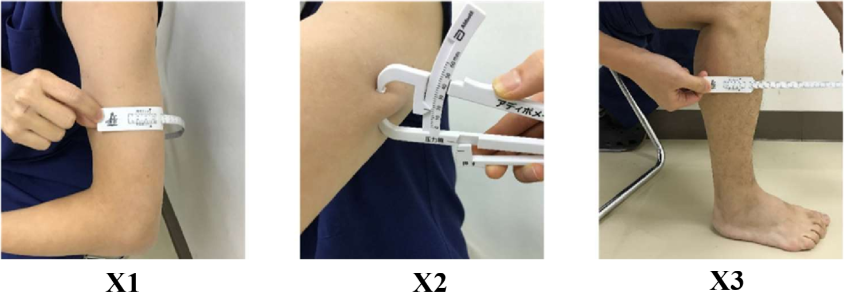
\includegraphics[scale=0.9]{X.png}
    \end{figure}

\end{frame}

% PART A.1 方法
\begin{frame}[t]{\textbf{PART A.1}}
\linespread{1.5}
{\Large \setlength{\baselineskip}{20pt} \parbox{\linewidth}{\raggedright \textbf{方法}}}
\begin{itemize}
    \item 多元線性迴歸
    \begin{enumerate}[]
        \item 建立 $Y = \beta_0+\beta_1X_1+\beta_2X_2+\beta_3X_3+\epsilon$

    \end{enumerate}

\end{itemize}
   

\end{frame}

% PART A.1 結果 (1)
\begin{frame}[t]{\textbf{PART A.1}}
\vspace*{10pt}
{\Large \setlength{\baselineskip}{20pt} \parbox{\linewidth}{\raggedright \textbf{結果 (1)}}}
\vspace*{10pt}
\begin{table}
\centering
\begin{tabular}{lrrrr}
\hline
Term & Estimate & Std.Err & t & p \\
\hline
Intercept        & 117.0847 & 99.7824 & 1.1734 & 0.2578 \\
Triceps (mm)     &   4.3341 &  3.0155 & 1.4373 & 0.1699 \\
Thigh (cm)       &  -2.8568 &  2.5820 & -1.1064 & 0.2849 \\
Midarm (cm)      &  -2.1861 &  1.5955 & -1.3701 & 0.1896 \\
\hline
\end{tabular}
\end{table}

\begin{itemize}
\item Adjusted $R^2 = 0.7641$
\item AIC = 98.62,\;\; BIC = 103.60
\end{itemize}

\end{frame}

% PART A.1 結果 (2)
\begin{frame}[t]{\textbf{PART A.1}}
\vspace*{10pt}
{\Large \setlength{\baselineskip}{20pt} \parbox{\linewidth}{\raggedright \textbf{結果 (2)}}}

\centering
\begin{figure}
    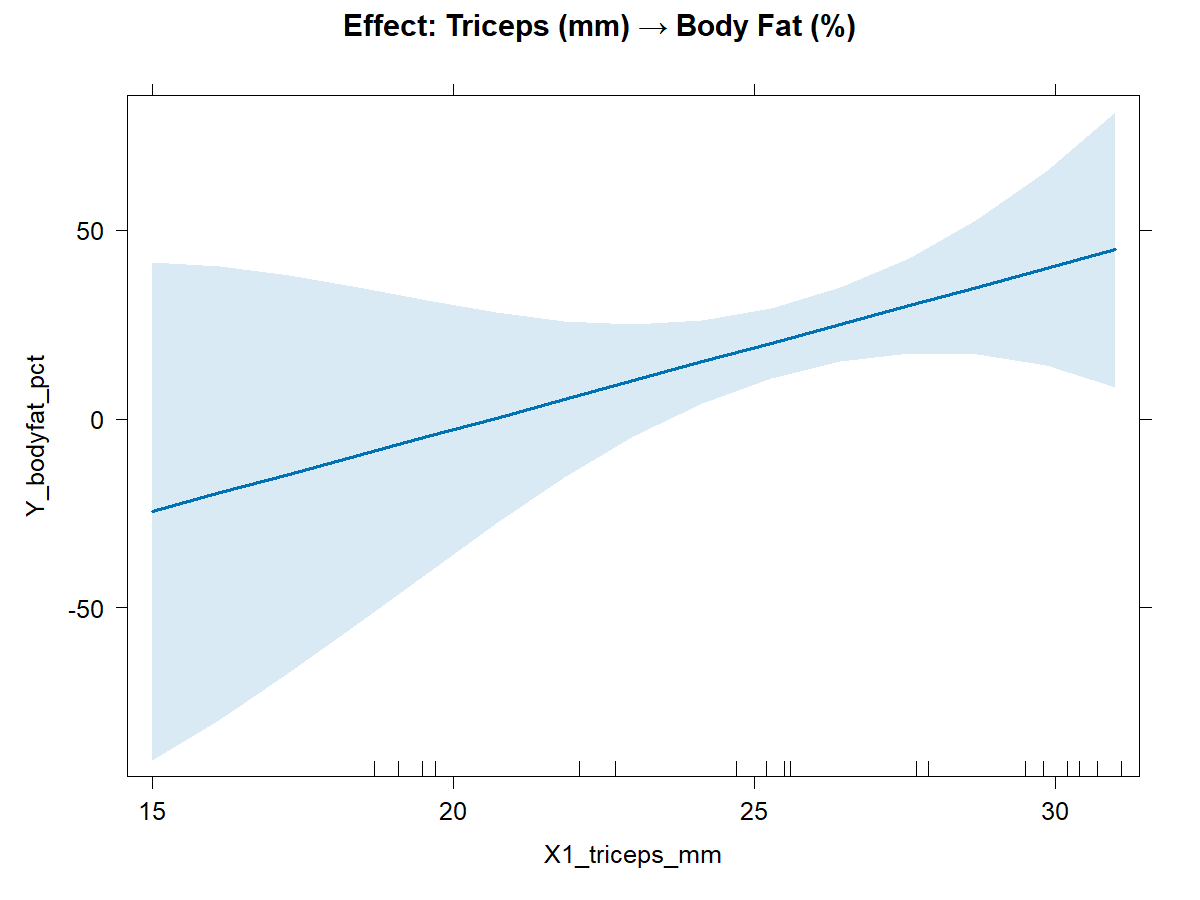
\includegraphics[width=0.32\textwidth]{PartA1_bodyfat_effect_X1.png}
    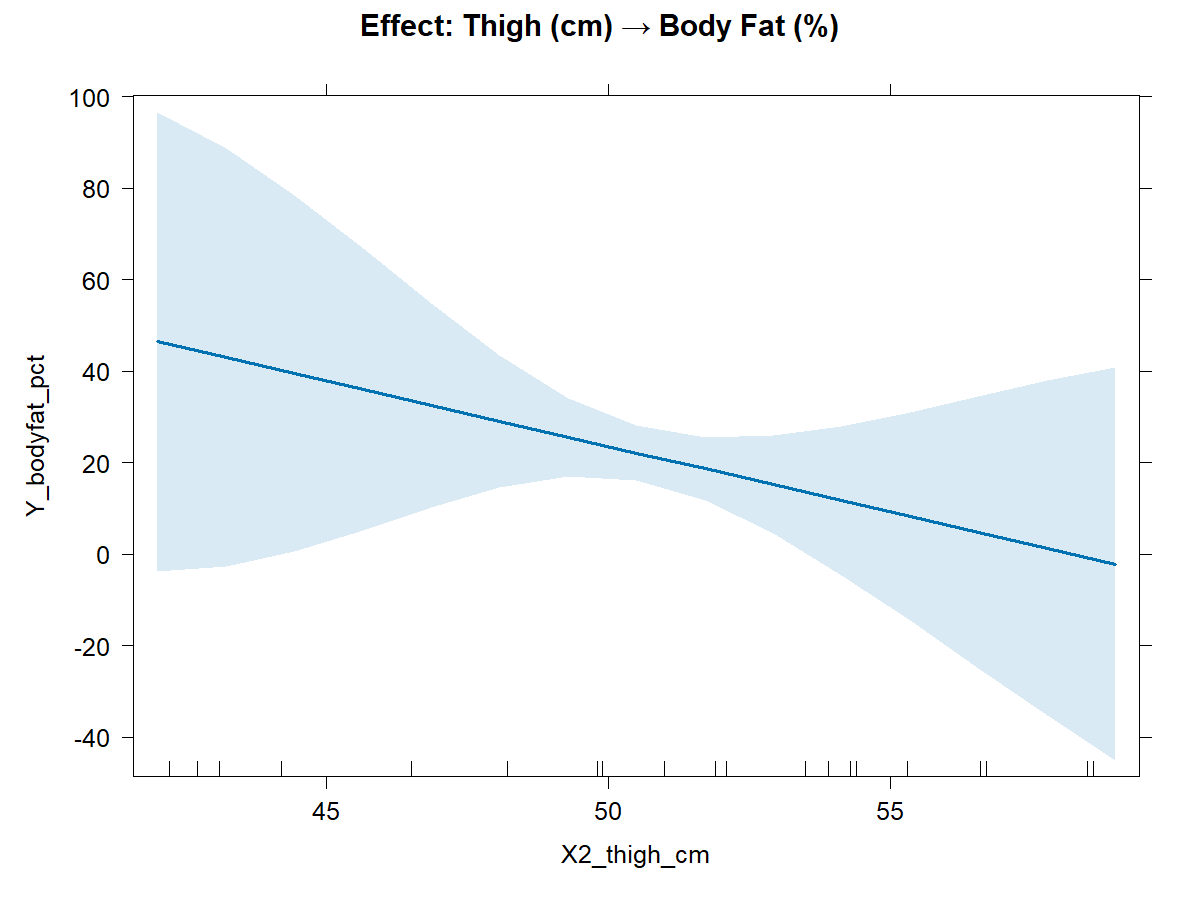
\includegraphics[width=0.32\textwidth]{PartA1_bodyfat_effect_X2.png}
    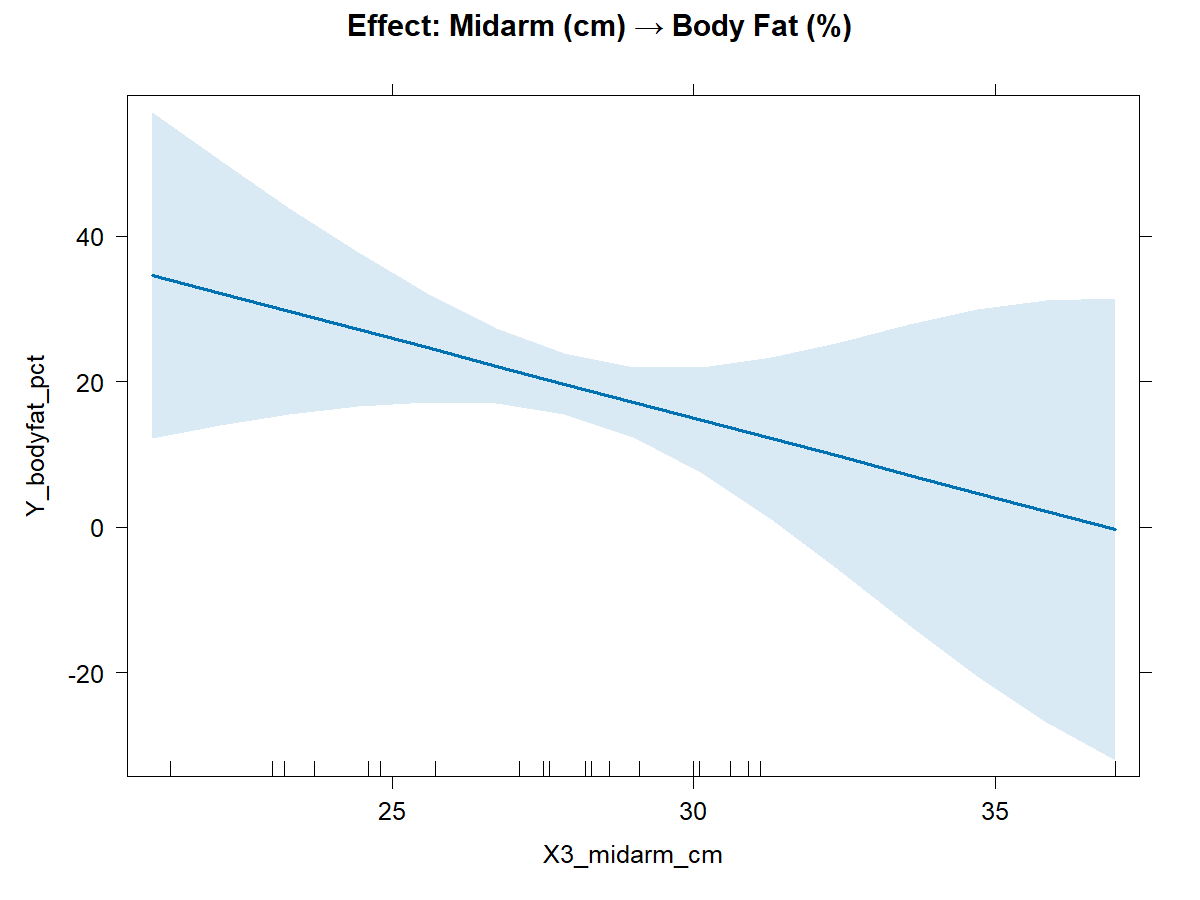
\includegraphics[width=0.32\textwidth]{PartA1_bodyfat_effect_X3.png}
\end{figure}

\begin{itemize}
\setlength{\itemsep}{10pt}
\item 三種量測在資料的中間值穩定，但在兩端的估計不穩定
\end{itemize}

\end{frame}

% PART A.1 結果 (3)
\begin{frame}[t]{\textbf{PART A.1}}
\vspace*{10pt}
{\Large \setlength{\baselineskip}{20pt} \parbox{\linewidth}{\raggedright \textbf{結果 (3)}}}

\centering
\begin{figure}
    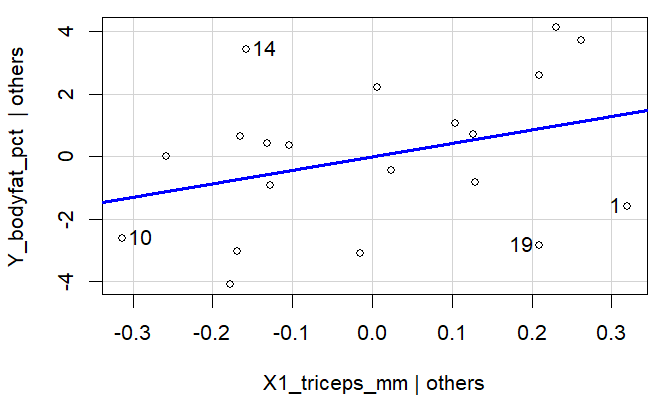
\includegraphics[width=0.32\textwidth]{PartA1_bodyfat_avplots_X1.png}
    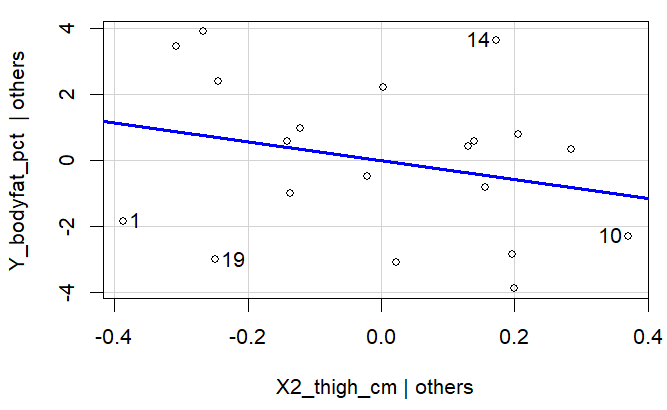
\includegraphics[width=0.32\textwidth]{PartA1_bodyfat_avplots_X2.png}
    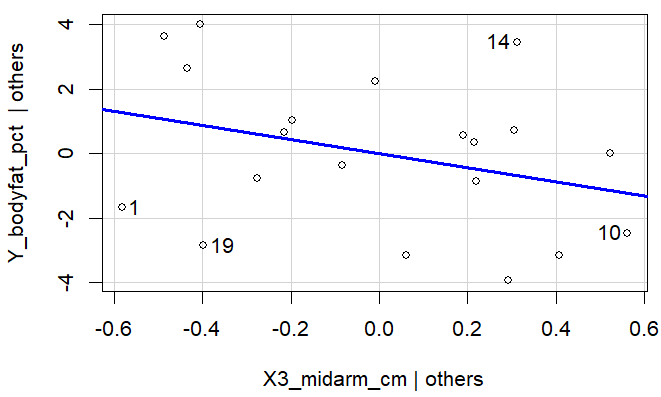
\includegraphics[width=0.32\textwidth]{PartA1_bodyfat_avplots_X3.png}
\end{figure}

\begin{itemize}
\setlength{\itemsep}{10pt}
\item 固定其他兩個變數下，三種量測的偏迴歸斜率皆接近水平
\end{itemize}

\end{frame}

% PART A.1 診斷
\begin{frame}[t]{\textbf{PART A.1}}
\vspace*{10pt}
{\Large \setlength{\baselineskip}{20pt} \parbox{\linewidth}{\raggedright \textbf{診斷}}}

% ----------- 左右併排 -----------
\begin{center}
\begin{minipage}{0.58\linewidth}   % 左：放大你的圖
\centering
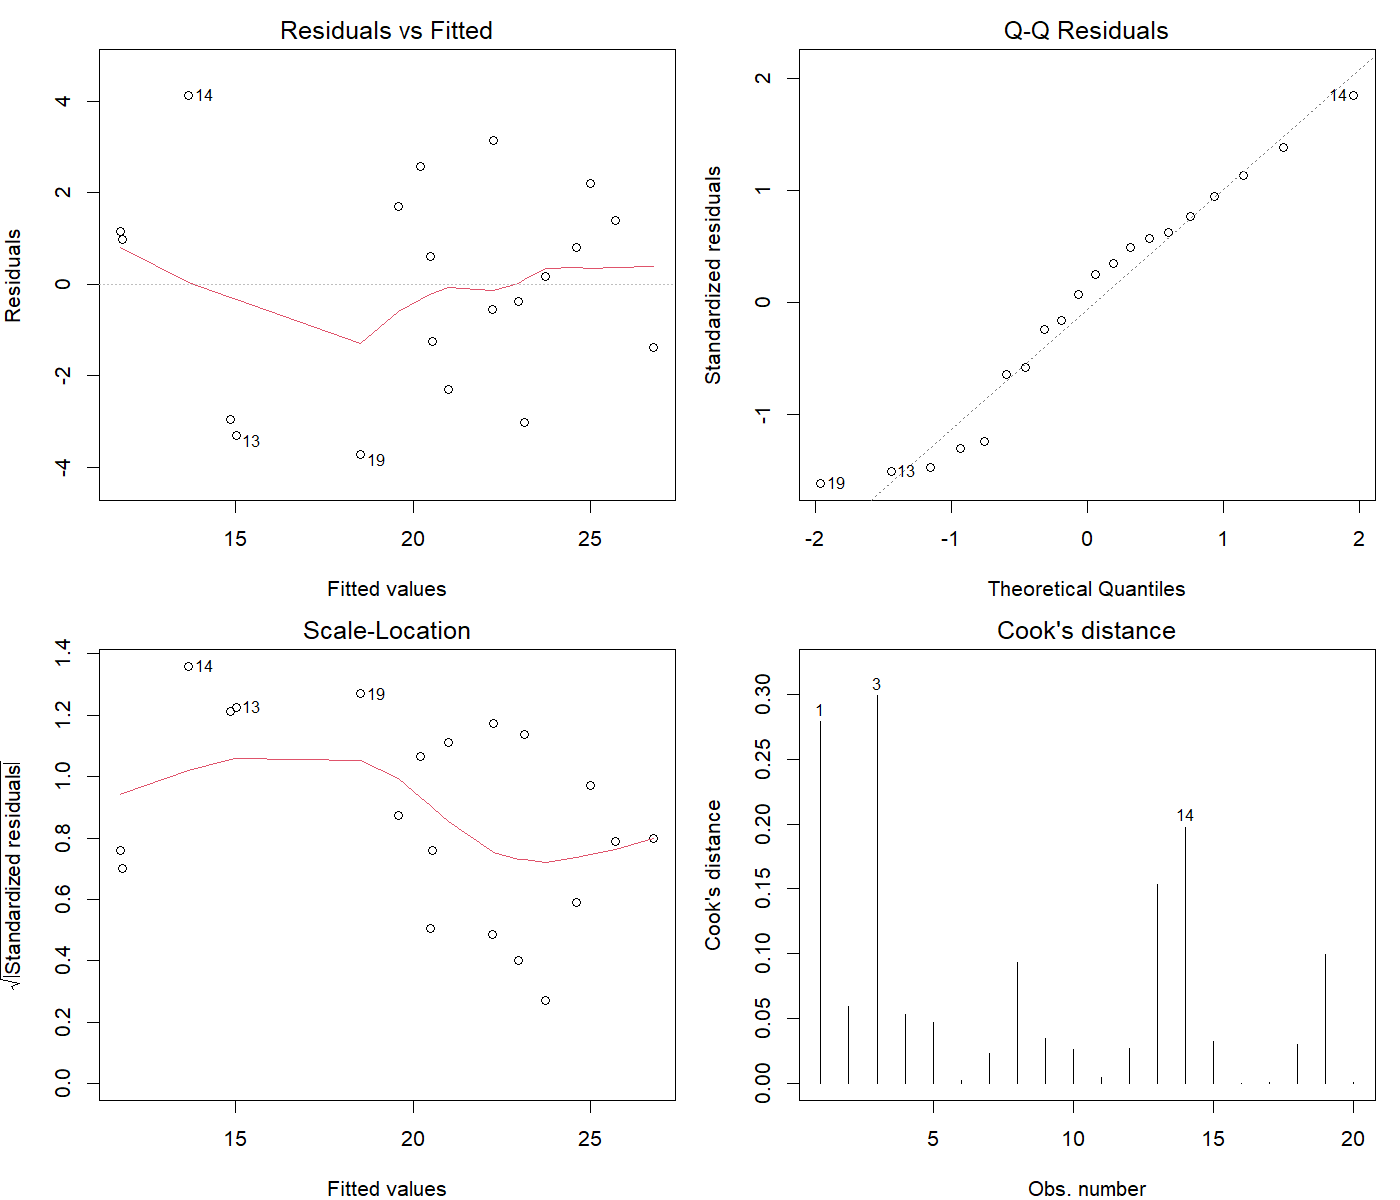
\includegraphics[width=1.1\linewidth]{PartA1_bodyfat_residuals.png}
\end{minipage}
\hfill
\begin{minipage}{0.35\linewidth}   % 右：縮小表格
\centering
\footnotesize
\begin{tabular}{lr}
\hline
Variable & VIF \\
\hline
Triceps (mm) & 708.843 \\
Thigh (cm)   & 564.343 \\
Midarm (cm)  & 104.606 \\
\hline
\end{tabular}
\end{minipage}
\end{center}

\end{frame}

% PART A.2 結論
\begin{frame}[t]{\textbf{PART A.1}}
\vspace*{10pt}
{\Large \setlength{\baselineskip}{20pt} \parbox{\linewidth}{\raggedright \textbf{結論}}}
\begin{itemize}
\setlength{\itemsep}{10pt}
\item 三個變數對體脂肪的可解釋程度達到近8成
\item 三個變數的共線性過高，對體脂肪的貢獻相當
\end{itemize}
\vspace*{30pt}

{\Large \setlength{\baselineskip}{20pt} \parbox{\linewidth}{\raggedright \textbf{下一步}}}
\begin{itemize}
\setlength{\itemsep}{10pt}
\item 選其中一項成本低或最容易操作的即可
\item 加入其他身體量測作為新變數
\end{itemize}
\textbf{}

\end{frame}

% PART A.2 問題與目的
\begin{frame}[t]{\textbf{PART A.2}}
\vspace*{10pt}

{
\setlength{\baselineskip}{1.5\baselineskip}
% 問題
{
\Large
\parbox{\linewidth}{\raggedright \textbf{問題}\\
評估三種媒體預算對產品銷售量的邊際效應與貢獻}
}

\vspace*{2cm}

% 目的
{
\Large \parbox{\linewidth}{\raggedright \textbf{目的}\\
找出哪個媒體預算對產品銷售量的影響最大且顯著}
}
}
\end{frame}

% PART A.2 資料
\begin{frame}[t]{\textbf{PART A.2}} 
\vspace*{10pt}
{
\setlength{\baselineskip}{1.3\baselineskip}   % 行距放大 1.3 倍
{
\Large
\parbox{\linewidth}{\raggedright \textbf{資料來源}}
}
}

\begin{itemize}
    \item Advertising.csv
  \begin{enumerate}[]
    \setlength{\itemsep}{6pt}
    \item 樣本數：200（收錄公司在三種媒體上的廣告支出與銷售成效）
    \item 研究變數：$X_1$：tv，$X_2$：radio，$X_3$：newspaper（千元）
    \item 目標變數：$Y$：sales（千件）
  \end{enumerate}
\end{itemize}

\vspace{0.5cm}

    \begin{center}
        
\includegraphics[scale=0.35]{Y.png}
    \end{center}

\end{frame}

% PART A.2 方法
\begin{frame}[t]{\textbf{PART A.2}}
\linespread{1.5}
{\Large \setlength{\baselineskip}{20pt} \parbox{\linewidth}{\raggedright \textbf{方法}}}
\begin{itemize}
    \item 多元線性迴歸
    \begin{enumerate}[]
        \item 建立 $Y = \beta_0+\beta_1X_1+\beta_2X_2+\beta_3X_3+\epsilon$

    \end{enumerate}

\end{itemize}
   

\end{frame}

% PART A.2 結果 (1)
\begin{frame}[t]{\textbf{PART A.2}}
\vspace*{10pt}
{\Large \setlength{\baselineskip}{20pt} \parbox{\linewidth}{\raggedright \textbf{結果 (1)}}}
\vspace*{10pt}
\begin{table}
\centering
\begin{tabular}{lrrrr}
\hline
Term & Estimate & Std.Err & t & p \\
\hline
Intercept        & 2.9389 & 0.3119 & 9.4223 & 0.0000 \\
tv    &   0.0458 &  0.0014 & 32.8086 & 0.0000 \\
radio       &  0.1885 &  0.0086 & 21.8935 & 0.0000 \\
newspaper    &  -0.0010 &  0.0059 & -0.1767 & 0.0000 \\
\hline
\end{tabular}
\end{table}

\begin{itemize}
\item Adjusted $R^2 = 0.8956$
\item AIC = 782.36,\;\; BIC = 798.85
\end{itemize}

\end{frame}

% PART A.2 結果 (2)
\begin{frame}[t]{\textbf{PART A.2}}
\vspace*{10pt}
{\Large \setlength{\baselineskip}{20pt} \parbox{\linewidth}{\raggedright \textbf{結果 (2)}}}

\centering
\begin{figure}
    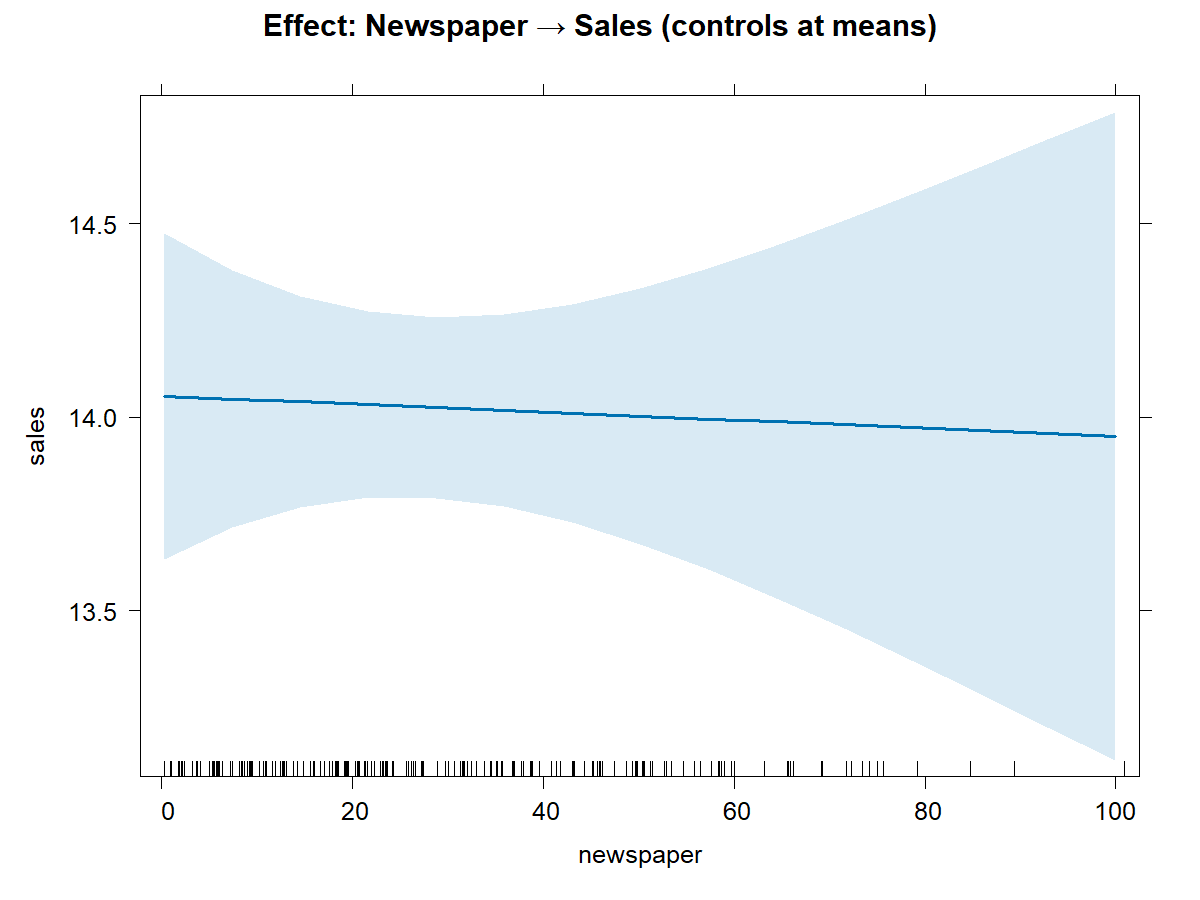
\includegraphics[width=0.32\textwidth]{PartA2_adv_effect_newspaper.png}
    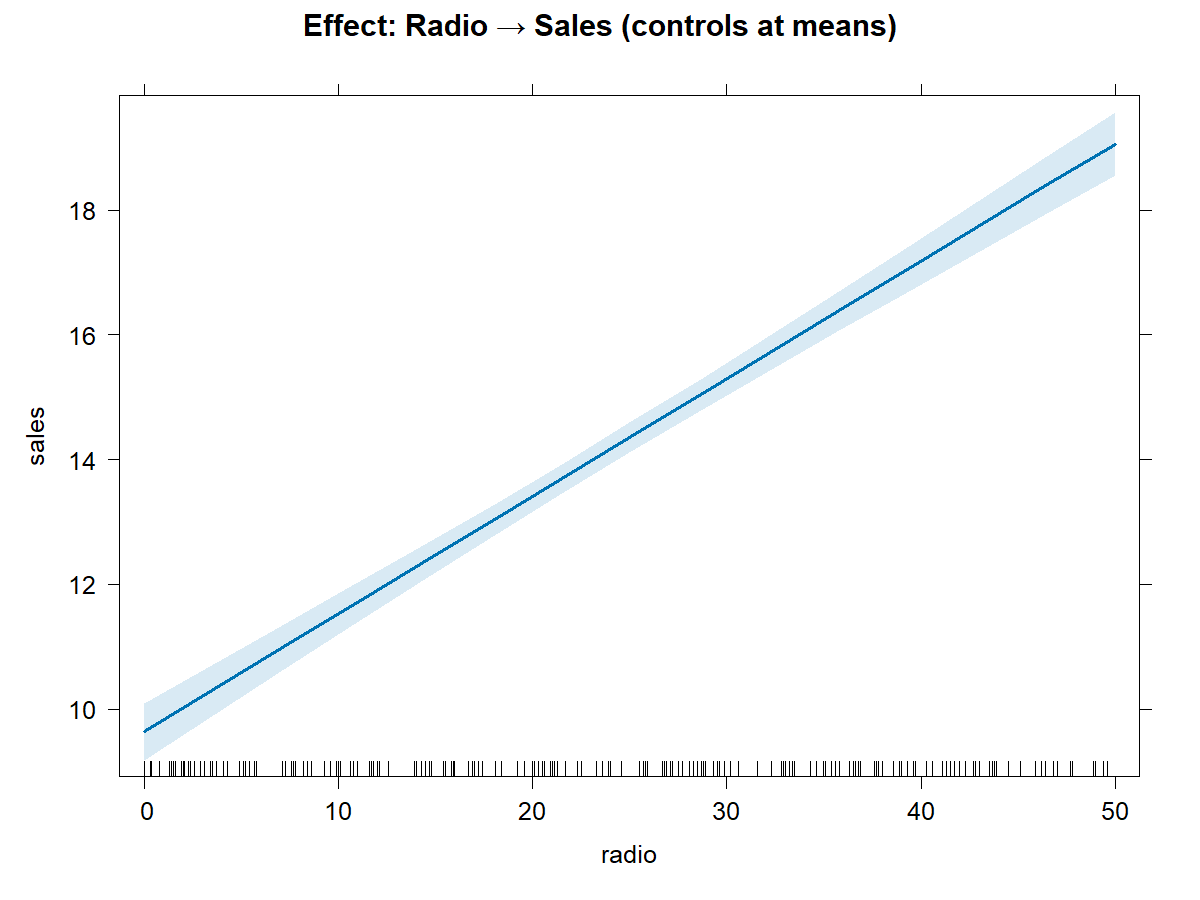
\includegraphics[width=0.32\textwidth]{PartA2_adv_effect_radio.png}
    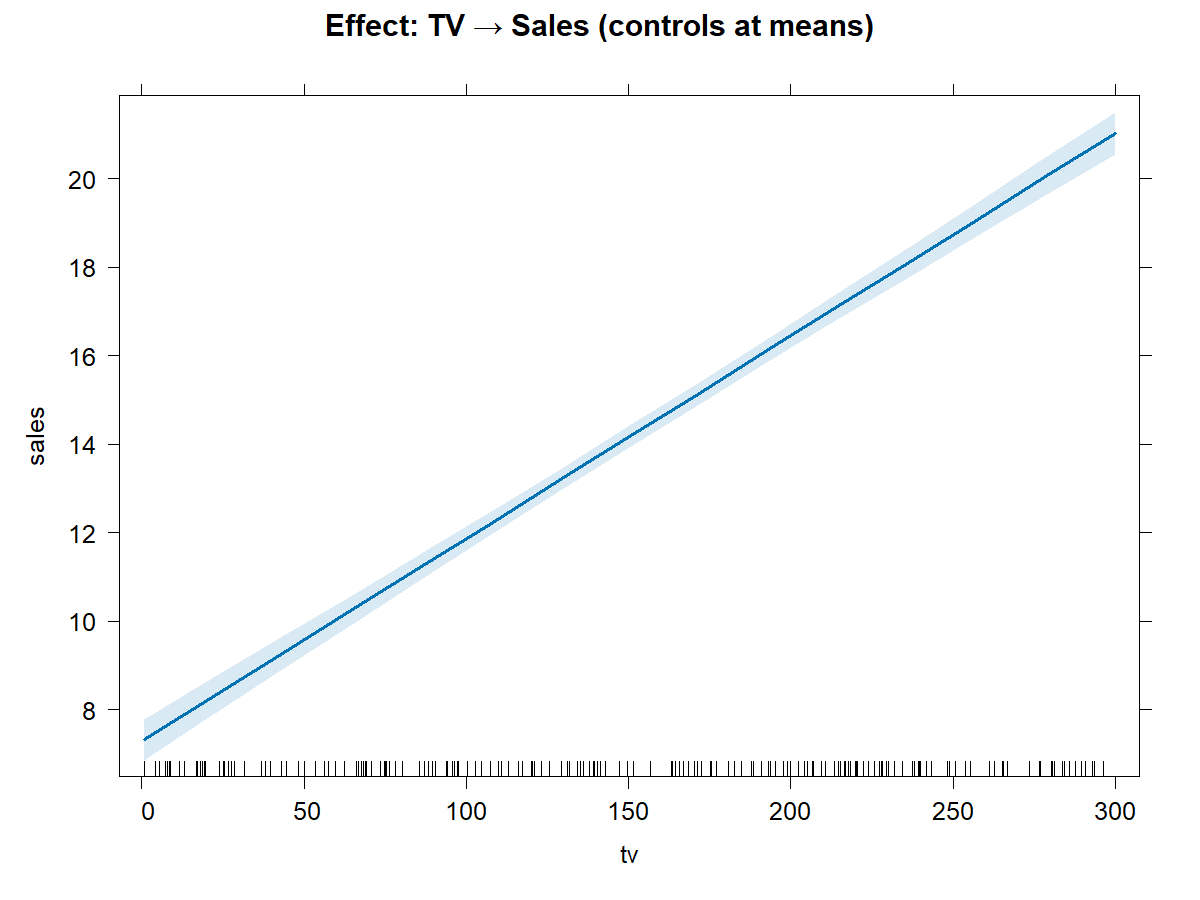
\includegraphics[width=0.32\textwidth]{PartA2_adv_effect_tv.png}
\end{figure}

\begin{itemize}
\setlength{\itemsep}{10pt}
\item 電視和廣播對銷售的估計穩定且顯著的正向邊際效應
\item 報紙的估計不穩定且邊際效應近乎為0
\end{itemize}

\end{frame}

% PART A.2 結果 (3)
\begin{frame}[t]{\textbf{PART A.2}}
\vspace*{10pt}
{\Large \setlength{\baselineskip}{20pt} \parbox{\linewidth}{\raggedright \textbf{結果 (3)}}}

\centering
\begin{figure}
    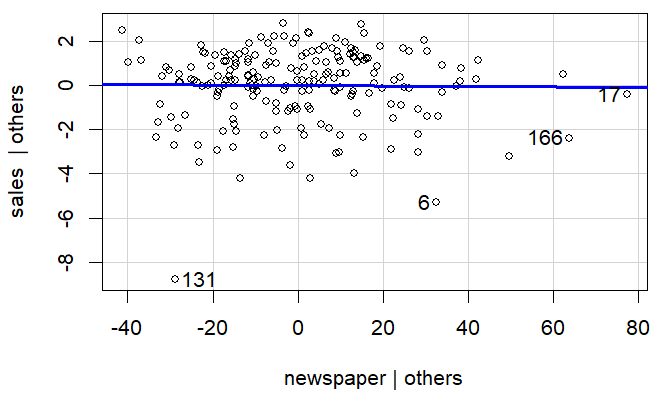
\includegraphics[width=0.32\textwidth]{PartA2_adv_avplots_newspaper.png}
    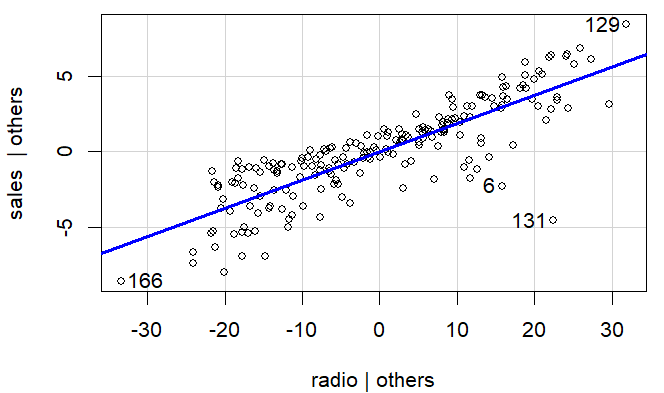
\includegraphics[width=0.32\textwidth]{PartA2_adv_avplots_radio.png}
    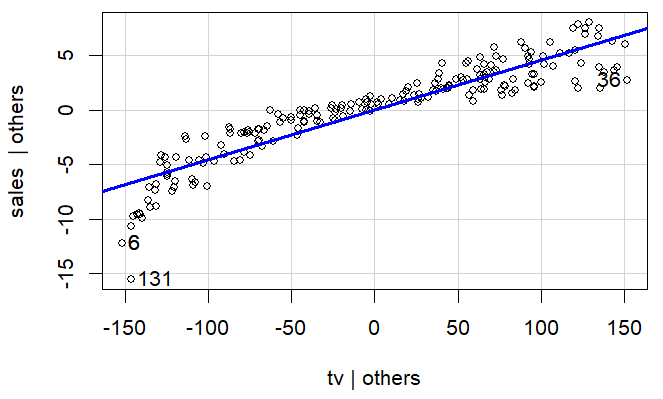
\includegraphics[width=0.32\textwidth]{PartA2_adv_avplots_tv.png}
\end{figure}

\begin{itemize}
\item 固定其他兩個變數下，三種廣告中，以TV和Radio的增加仍能提升銷售量，報紙則幾乎沒有影響
\end{itemize}

\end{frame}

% PART A.2 診斷
\begin{frame}[t]{\textbf{PART A.2}}
\vspace*{10pt}
{\Large \setlength{\baselineskip}{20pt} \parbox{\linewidth}{\raggedright \textbf{診斷}}}

\vspace*{15pt}
\begin{center}
\begin{itemize}
\item Shapiro--Wilk: $W=0.918$, $p=0.0000$
\item Breusch--Pagan: $BP=5.133$, $p=0.1623$
\end{itemize}
\vspace*{15pt}
\begin{tabular}{lr}
\hline
Variable & VIF \\
\hline
tv & 1.005 \\
radio   & 1.145 \\
newspaper & 1.145 \\
\hline
\end{tabular}

\end{center}

\end{frame}

% PART A.2 結論
\begin{frame}[t]{\textbf{PART A.2}}
\vspace*{10pt}
{\Large \setlength{\baselineskip}{20pt} \parbox{\linewidth}{\raggedright \textbf{結論}}}
\begin{itemize}
\setlength{\itemsep}{10pt}
\item 三個變數對產品銷售量的可解釋程度達到近9成
\item 電視廣告和廣播廣告，對產品銷售量有相當大的提升
\end{itemize}
\vspace*{30pt}

{\Large \setlength{\baselineskip}{20pt} \parbox{\linewidth}{\raggedright \textbf{下一步}}}
\begin{itemize}
\setlength{\itemsep}{10pt}
\item 增加電視廣告和廣播廣告的預算
\item 考慮刪除報紙廣告的預算
\end{itemize}
\textbf{}

\end{frame}

% PART B 問題與目的
\begin{frame}[t]{\textbf{PART B}}
\vspace*{10pt}

{
\setlength{\baselineskip}{1.5\baselineskip}
% 問題
{
\Large
\parbox{\linewidth}{\raggedright \textbf{問題}\\
年齡越高，五年內存活的機率是否越低}
}

\vspace*{2cm}

% 目的
{
\Large \parbox{\linewidth}{\raggedright \textbf{目的}\\
找出年齡與五年內存機率的相關性}
}
}
\end{frame}

% PART B 資料
\begin{frame}[t]{\textbf{PART B}} 
\vspace*{10pt}
{
\setlength{\baselineskip}{1.3\baselineskip}   % 行距放大 1.3 倍
{
\Large
\parbox{\linewidth}{\raggedright \textbf{資料來源}}
}
}

\begin{itemize}
    \item Melanoma
  \begin{enumerate}[]
    \setlength{\itemsep}{6pt}
    \item 樣本數：205（黑色素瘤臨床資料）
    \item 研究變數：$X_1$：age
    \item 目標變數：$Y_i=1$ if 五年內存活，$Y_i=0$ if 五年內死亡
  \end{enumerate}
\end{itemize}

\end{frame}

% PART B 方法
\begin{frame}[t]{\textbf{PART B}}
\linespread{1.5}
{\Large \setlength{\baselineskip}{20pt} \parbox{\linewidth}{\raggedright \textbf{方法}}}
\begin{itemize}
    \item Logistic regression
    \begin{enumerate}[]
        \item 建立 $logit(p_i) = \beta_0+\beta_1X_1$，其中 $p_i$為存活至少五年的機率

    \end{enumerate}

\end{itemize}
   

\end{frame}

% PART B 結果 (1)
\begin{frame}[t]{\textbf{PART B}}
\vspace*{10pt}
{\Large \setlength{\baselineskip}{20pt} \parbox{\linewidth}{\raggedright \textbf{結果 (1)}}}
\vspace*{20pt}
\begin{itemize}
    \item 迴歸方程式：$\widehat{\text{logit}}(p_i)= 1.083 - 0.0197\,\text{age}_i.$
    \vspace*{10pt}
    \item 勝算比：$\text{OR} = e^{-0.0197} \approx 0.9805$
    \vspace*{5pt}
    \begin{enumerate}[]
        \item 信賴區間：$95\% \ \text{CI} = (0.964,\; 0.997)$
    \end{enumerate}
    \vspace*{10pt}
\end{itemize}

\end{frame}

% PART B 結果 (2)
\begin{frame}[t]{\textbf{PART B}}
\vspace*{10pt}
{\Large \setlength{\baselineskip}{20pt} \parbox{\linewidth}{\raggedright \textbf{結果 (2)}}}

    \begin{center}
        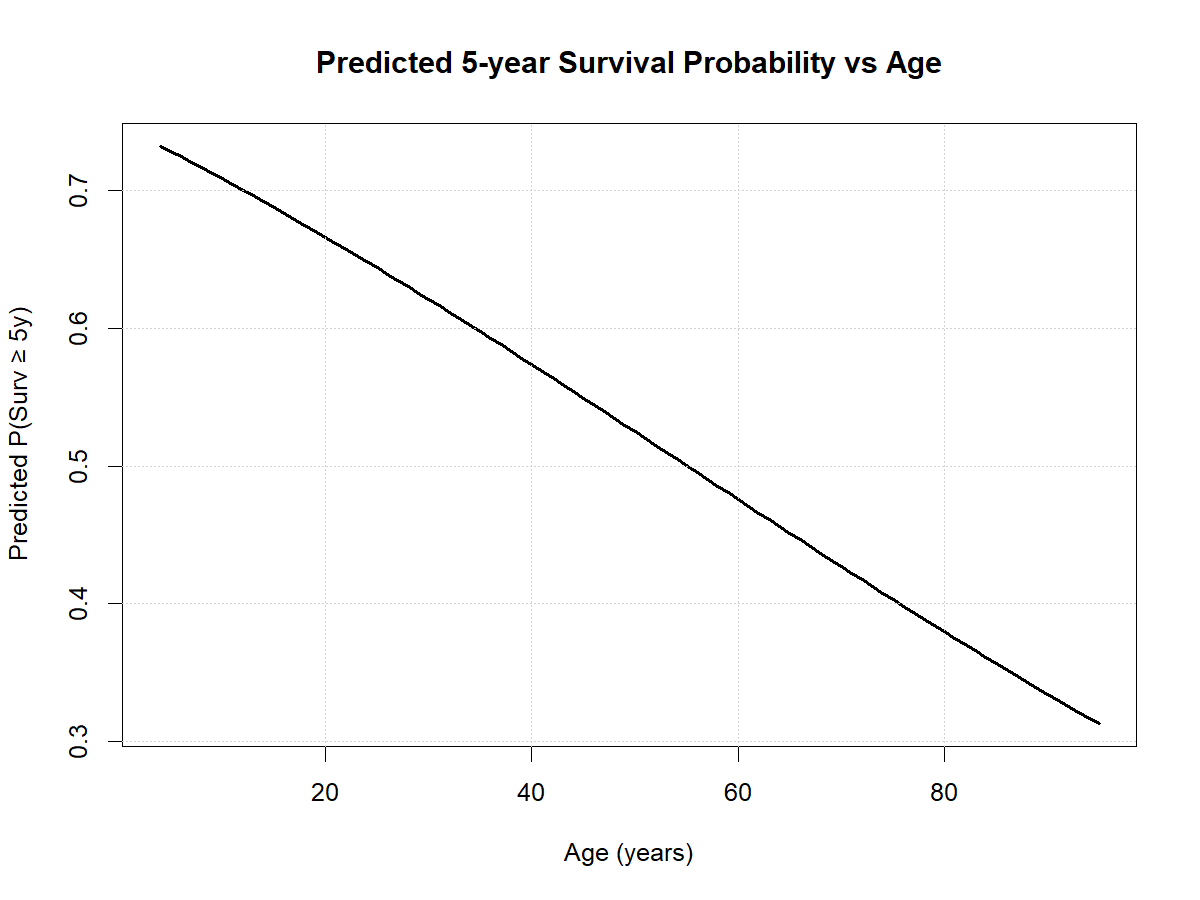
\includegraphics[scale=0.35]{PartB_logistic_curve.png}
    \end{center}

    \begin{itemize}
    \item 年齡與存活率呈現負相關
    \end{itemize}

\end{frame}

% PART B 結論
\begin{frame}[t]{\textbf{PART B}}
\vspace*{10pt}
{\Large \setlength{\baselineskip}{20pt} \parbox{\linewidth}{\raggedright \textbf{結論}}}
\begin{itemize}
    \item 年齡每增加1歲，病患存活至少五年的勝算平均下降約1.95\%
    （$0.9805-1=-0.0195$）
    \vspace*{10pt}
    \item 隨著年齡增加，存活機率會逐漸降低
\end{itemize}

\vspace*{30pt}

{\Large \setlength{\baselineskip}{20pt} \parbox{\linewidth}{\raggedright \textbf{下一步}}}
\begin{itemize}
\setlength{\itemsep}{10pt}
\item 增加其他病因或相關症狀的診斷，建立更完整的預測模型
\end{itemize}
\textbf{}

\end{frame}

% END
\begin{frame}[plain] % 產生無外框的頁面
	\begin{center}
		{\Huge The End}
		\bigskip\bigskip 
		
		{\LARGE Questions}
	\end{center}
\end{frame}
\end{document}
